\documentclass{article}\usepackage[]{graphicx}\usepackage[]{color}
%% maxwidth is the original width if it is less than linewidth
%% otherwise use linewidth (to make sure the graphics do not exceed the margin)
\makeatletter
\def\maxwidth{ %
  \ifdim\Gin@nat@width>\linewidth
    \linewidth
  \else
    \Gin@nat@width
  \fi
}
\makeatother

\definecolor{fgcolor}{rgb}{0.345, 0.345, 0.345}
\newcommand{\hlnum}[1]{\textcolor[rgb]{0.686,0.059,0.569}{#1}}%
\newcommand{\hlstr}[1]{\textcolor[rgb]{0.192,0.494,0.8}{#1}}%
\newcommand{\hlcom}[1]{\textcolor[rgb]{0.678,0.584,0.686}{\textit{#1}}}%
\newcommand{\hlopt}[1]{\textcolor[rgb]{0,0,0}{#1}}%
\newcommand{\hlstd}[1]{\textcolor[rgb]{0.345,0.345,0.345}{#1}}%
\newcommand{\hlkwa}[1]{\textcolor[rgb]{0.161,0.373,0.58}{\textbf{#1}}}%
\newcommand{\hlkwb}[1]{\textcolor[rgb]{0.69,0.353,0.396}{#1}}%
\newcommand{\hlkwc}[1]{\textcolor[rgb]{0.333,0.667,0.333}{#1}}%
\newcommand{\hlkwd}[1]{\textcolor[rgb]{0.737,0.353,0.396}{\textbf{#1}}}%
\let\hlipl\hlkwb

\usepackage{framed}
\makeatletter
\newenvironment{kframe}{%
 \def\at@end@of@kframe{}%
 \ifinner\ifhmode%
  \def\at@end@of@kframe{\end{minipage}}%
  \begin{minipage}{\columnwidth}%
 \fi\fi%
 \def\FrameCommand##1{\hskip\@totalleftmargin \hskip-\fboxsep
 \colorbox{shadecolor}{##1}\hskip-\fboxsep
     % There is no \\@totalrightmargin, so:
     \hskip-\linewidth \hskip-\@totalleftmargin \hskip\columnwidth}%
 \MakeFramed {\advance\hsize-\width
   \@totalleftmargin\z@ \linewidth\hsize
   \@setminipage}}%
 {\par\unskip\endMakeFramed%
 \at@end@of@kframe}
\makeatother

\definecolor{shadecolor}{rgb}{.97, .97, .97}
\definecolor{messagecolor}{rgb}{0, 0, 0}
\definecolor{warningcolor}{rgb}{1, 0, 1}
\definecolor{errorcolor}{rgb}{1, 0, 0}
\newenvironment{knitrout}{}{} % an empty environment to be redefined in TeX

\usepackage{alltt}

\usepackage{hyperref}

\title{Package \textbf{CompSign}}
\author{Lena Morrill}
\date{October 2017}
\IfFileExists{upquote.sty}{\usepackage{upquote}}{}
\begin{document}

\maketitle

\textbf{CompSign} is a package for yadayada... overlooked that mutational signatures are compositional in nature yadayada. The reference manual can be found \href{https://github.com/lm687/CompSign/blob/master/CompSign.pdf}{here}.

\begin{knitrout}
\definecolor{shadecolor}{rgb}{0.969, 0.969, 0.969}\color{fgcolor}\begin{kframe}
\begin{alltt}
\hlstd{knitr}\hlopt{::}\hlstd{opts_chunk}\hlopt{$}\hlkwd{set}\hlstd{(}\hlkwc{cache} \hlstd{=} \hlnum{FALSE}\hlstd{)}
\end{alltt}
\end{kframe}
\end{knitrout}

\begin{knitrout}
\definecolor{shadecolor}{rgb}{0.969, 0.969, 0.969}\color{fgcolor}\begin{kframe}
\begin{alltt}
\hlcom{## This chunk was last ran in}
\hlkwd{timestamp}\hlstd{()}
\end{alltt}
\begin{verbatim}
## ##------ Wed Nov  7 09:53:08 2018 ------##
\end{verbatim}
\begin{alltt}
\hlcom{## install latest version}
\hlkwd{library}\hlstd{(devtools)}
\hlstd{devtools}\hlopt{::}\hlkwd{install_github}\hlstd{(}\hlstr{"lm687/CompSign"}\hlstd{)}
\end{alltt}


{\ttfamily\noindent\itshape\color{messagecolor}{\#\# Downloading GitHub repo lm687/CompSign@master}}\begin{verbatim}
## 
##   
   checking for file ‘/private/var/folders/22/gyg0hl2s7f73m8f05lb35080qz1b0n/T/RtmpQrj6E4/remotes3cb20486ec8/lm687-CompSign-5d2fe49/DESCRIPTION’ ...
  
v  checking for file ‘/private/var/folders/22/gyg0hl2s7f73m8f05lb35080qz1b0n/T/RtmpQrj6E4/remotes3cb20486ec8/lm687-CompSign-5d2fe49/DESCRIPTION’ (464ms)
## 
  
-  preparing ‘CompSign’:
## 
  
   checking DESCRIPTION meta-information ...
  
v  checking DESCRIPTION meta-information
## 
  
  
  
-  excluding invalid files
## 
  
   Subdirectory 'man' contains invalid file names:
##      ‘summary_ROO.txt’
## 
  
-  checking for LF line-endings in source and make files and shell scripts
## 
  
-  checking for empty or unneeded directories
## 
  
-  building ‘CompSign_0.1.0.tar.gz’
## 
  
   Warning: invalid uid value replaced by that for user 'nobody'
## 
  
   
## 
\end{verbatim}
\begin{alltt}
\hlkwd{library}\hlstd{(CompSign)}
\hlkwd{library}\hlstd{(compositions)}
\end{alltt}


{\ttfamily\noindent\itshape\color{messagecolor}{\#\# Loading required package: tensorA}}

{\ttfamily\noindent\itshape\color{messagecolor}{\#\# \\\#\# Attaching package: 'tensorA'}}

{\ttfamily\noindent\itshape\color{messagecolor}{\#\# The following object is masked from 'package:base':\\\#\# \\\#\#\ \ \ \  norm}}

{\ttfamily\noindent\itshape\color{messagecolor}{\#\# Loading required package: robustbase}}

{\ttfamily\noindent\itshape\color{messagecolor}{\#\# Loading required package: energy}}

{\ttfamily\noindent\itshape\color{messagecolor}{\#\# Loading required package: bayesm}}

{\ttfamily\noindent\itshape\color{messagecolor}{\#\# Welcome to compositions, a package for compositional data analysis.\\\#\# Find an intro with "{}? compositions"{}}}

{\ttfamily\noindent\itshape\color{messagecolor}{\#\# \\\#\# Attaching package: 'compositions'}}

{\ttfamily\noindent\itshape\color{messagecolor}{\#\# The following objects are masked from 'package:stats':\\\#\# \\\#\#\ \ \ \  cor, cov, dist, var}}

{\ttfamily\noindent\itshape\color{messagecolor}{\#\# The following objects are masked from 'package:base':\\\#\# \\\#\#\ \ \ \  \%*\%, scale, scale.default}}\end{kframe}
\end{knitrout}

\begin{knitrout}
\definecolor{shadecolor}{rgb}{0.969, 0.969, 0.969}\color{fgcolor}\begin{kframe}
\begin{alltt}
\hlcom{## This chunk was last ran in}
\hlkwd{timestamp}\hlstd{()}
\end{alltt}
\begin{verbatim}
## ##------ Wed Nov  7 09:53:38 2018 ------##
\end{verbatim}
\begin{alltt}
\hlcom{##########################}
\hlcom{####### Dummy data #######}
\hlcom{##########################}

\hlcom{### Example of matrix transformed into sign object}
\hlstd{input_dummy} \hlkwb{<-} \hlkwd{matrix}\hlstd{(}\hlkwd{runif}\hlstd{(}\hlnum{100}\hlstd{),} \hlnum{4}\hlstd{)}
\hlkwd{colnames}\hlstd{(input_dummy)} \hlkwb{<-} \hlkwd{paste0}\hlstd{(}\hlstr{'s'}\hlstd{,} \hlnum{1}\hlopt{:}\hlnum{25}\hlstd{);} \hlkwd{rownames}\hlstd{(input_dummy)} \hlkwb{<-} \hlkwd{paste0}\hlstd{(}\hlstr{'sam'}\hlstd{,} \hlnum{1}\hlopt{:}\hlnum{4}\hlstd{)}
\hlstd{sign_dummy} \hlkwb{<-} \hlkwd{to_sign}\hlstd{(input_dummy)}
\end{alltt}
\end{kframe}
\end{knitrout}

\section{Summarise the signature matrix}
\begin{knitrout}
\definecolor{shadecolor}{rgb}{0.969, 0.969, 0.969}\color{fgcolor}\begin{kframe}
\begin{alltt}
\hlcom{## This chunk was last ran in}
\hlkwd{timestamp}\hlstd{()}
\end{alltt}
\begin{verbatim}
## ##------ Wed Nov  7 09:53:38 2018 ------##
\end{verbatim}
\begin{alltt}
\hlkwd{add_together_matrix}\hlstd{(sign_dummy)}
\end{alltt}
\begin{verbatim}
## An object of class "sign"
## Slot "id":
## [1] "input_dummy"
## 
## Slot "id_samples":
## [1] "sam1" "sam2" "sam3" "sam4"
## 
## Slot "id_signatures":
##  [1] "s1"  "s2"  "s3"  "s4"  "s5"  "s6"  "s7"  "s8"  "s9"  "s10" "s11"
## [12] "s12" "s13" "s14" "s15" "s16" "s17" "s18" "s19" "s20" "s21" "s22"
## [23] "s23" "s24" "s25"
## 
## Slot "count_matrix":
##             s1        s2         s3        s4        s5         s6
## sam1 0.6130077 0.6201001 0.02548431 0.9164084 0.2908617 0.07488885
## sam2 0.9900551 0.3453004 0.80846802 0.6432645 0.7316618 0.92458896
## sam3 0.2915941 0.4309228 0.75626895 0.5831739 0.8232874 0.15455563
## sam4 0.7403550 0.3917636 0.78327104 0.4309776 0.1752640 0.94668388
##             s7        s8        s9        s10       s11       s12
## sam1 0.7811775 0.5824201 0.7072237 0.86595023 0.3520402 0.4358718
## sam2 0.5869432 0.6389264 0.3450403 0.07703436 0.4722528 0.7467841
## sam3 0.8196181 0.3919323 0.7823582 0.74613238 0.5338816 0.0846173
## sam4 0.7044953 0.3257368 0.9367393 0.99475854 0.9464276 0.5732689
##            s13       s14       s15       s16       s17       s18
## sam1 0.9754523 0.6971351 0.5247873 0.5126980 0.5080613 0.8311513
## sam2 0.5771914 0.9870072 0.4881304 0.8546315 0.5936254 0.6873601
## sam3 0.7392869 0.5104545 0.1886795 0.3496769 0.6928111 0.6738743
## sam4 0.9027598 0.3239889 0.9622762 0.2661097 0.3346391 0.6533321
##             s19       s20       s21       s22       s23       s24
## sam1 0.09571556 0.1549136 0.2458252 0.3138197 0.8134497 0.6355442
## sam2 0.42322630 0.7672090 0.9687606 0.3592505 0.9477584 0.7051245
## sam3 0.08214040 0.9420649 0.8997512 0.2251877 0.4940255 0.9120137
## sam4 0.91560367 0.1443106 0.7358621 0.9465534 0.3667558 0.2882320
##             s25
## sam1 0.07286385
## sam2 0.26951424
## sam3 0.64187211
## sam4 0.90365832
## 
## Slot "modified":
## [1] TRUE
\end{verbatim}
\begin{alltt}
\hlstd{results_sumarise} \hlkwb{<-} \hlkwd{summarise}\hlstd{(}\hlkwd{add_together_matrix}\hlstd{(sign_dummy))}
\hlstd{results_sumarise}\hlopt{$}\hlstd{General}
\end{alltt}
\begin{verbatim}
## [1] "Object of class sign"
\end{verbatim}
\end{kframe}
\end{knitrout}

\section{Linear model for numerical predictors}
\begin{knitrout}
\definecolor{shadecolor}{rgb}{0.969, 0.969, 0.969}\color{fgcolor}\begin{kframe}
\begin{alltt}
\hlcom{## This chunk was last ran in}
\hlkwd{timestamp}\hlstd{()}
\end{alltt}
\begin{verbatim}
## ##------ Wed Nov  7 09:53:38 2018 ------##
\end{verbatim}
\begin{alltt}
\hlstd{tmp_merged_compositional} \hlkwb{<-} \hlkwd{new}\hlstd{(}\hlstr{"merged_compositional"}\hlstd{,}
                                \hlkwc{id}\hlstd{=}\hlstr{'adas'}\hlstd{,}
                                \hlkwc{id_samples}\hlstd{=}\hlkwd{paste0}\hlstd{(}\hlstr{"sam"}\hlstd{,} \hlnum{1}\hlopt{:}\hlnum{30}\hlstd{),}
                                \hlkwc{id_signatures}\hlstd{=} \hlkwd{c}\hlstd{(}\hlstr{'s1'}\hlstd{,} \hlstr{'s2'}\hlstd{,} \hlstr{'s3'}\hlstd{,} \hlstr{'s4'}\hlstd{),} \hlcom{## signature names}
                                \hlkwc{count_matrix}\hlstd{=MCMCpack}\hlopt{::}\hlkwd{rdirichlet}\hlstd{(}\hlnum{30}\hlstd{,} \hlkwd{c}\hlstd{(}\hlnum{1}\hlstd{,}\hlnum{1}\hlstd{,}\hlnum{1}\hlstd{,}\hlnum{1}\hlstd{)),}
                                \hlkwc{df}\hlstd{=}\hlkwd{data.frame}\hlstd{(}\hlkwc{a}\hlstd{=}\hlkwd{sample}\hlstd{(}\hlnum{1}\hlopt{:}\hlnum{1e4}\hlstd{,} \hlnum{30}\hlstd{),} \hlkwc{b}\hlstd{=}\hlkwd{rep}\hlstd{(}\hlnum{10}\hlstd{,} \hlnum{30}\hlstd{)))}
\hlkwd{comp_lm}\hlstd{(tmp_merged_compositional)}
\end{alltt}
\begin{verbatim}
## [[1]]
## Response Y1 :
## 
## Call:
## lm(formula = Y1 ~ as.matrix((x@df)[, indices_predictor]))
## 
## Residuals:
##     Min      1Q  Median      3Q     Max 
## -1.8146 -0.7776  0.1236  0.6441  3.1480 
## 
## Coefficients: (1 not defined because of singularities)
##                                           Estimate Std. Error t value
## (Intercept)                              3.258e-01  4.733e-01   0.688
## as.matrix((x@df)[, indices_predictor])a -1.047e-04  8.822e-05  -1.187
## as.matrix((x@df)[, indices_predictor])b         NA         NA      NA
##                                         Pr(>|t|)
## (Intercept)                                0.497
## as.matrix((x@df)[, indices_predictor])a    0.245
## as.matrix((x@df)[, indices_predictor])b       NA
## 
## Residual standard error: 1.137 on 28 degrees of freedom
## Multiple R-squared:  0.04788,	Adjusted R-squared:  0.01388 
## F-statistic: 1.408 on 1 and 28 DF,  p-value: 0.2453
## 
## 
## Response Y2 :
## 
## Call:
## lm(formula = Y2 ~ as.matrix((x@df)[, indices_predictor]))
## 
## Residuals:
##     Min      1Q  Median      3Q     Max 
## -2.4838 -1.1343  0.1275  1.1752  2.0129 
## 
## Coefficients: (1 not defined because of singularities)
##                                           Estimate Std. Error t value
## (Intercept)                             -1.0767141  0.5460040  -1.972
## as.matrix((x@df)[, indices_predictor])a  0.0002004  0.0001018   1.969
## as.matrix((x@df)[, indices_predictor])b         NA         NA      NA
##                                         Pr(>|t|)  
## (Intercept)                               0.0586 .
## as.matrix((x@df)[, indices_predictor])a   0.0589 .
## as.matrix((x@df)[, indices_predictor])b       NA  
## ---
## Signif. codes:  0 '***' 0.001 '**' 0.01 '*' 0.05 '.' 0.1 ' ' 1
## 
## Residual standard error: 1.312 on 28 degrees of freedom
## Multiple R-squared:  0.1216,	Adjusted R-squared:  0.09027 
## F-statistic: 3.878 on 1 and 28 DF,  p-value: 0.0589
## 
## 
## Response Y3 :
## 
## Call:
## lm(formula = Y3 ~ as.matrix((x@df)[, indices_predictor]))
## 
## Residuals:
##      Min       1Q   Median       3Q      Max 
## -2.22997 -0.43382  0.07819  0.67836  1.85067 
## 
## Coefficients: (1 not defined because of singularities)
##                                           Estimate Std. Error t value
## (Intercept)                              7.110e-01  3.814e-01   1.864
## as.matrix((x@df)[, indices_predictor])a -1.294e-04  7.109e-05  -1.821
## as.matrix((x@df)[, indices_predictor])b         NA         NA      NA
##                                         Pr(>|t|)  
## (Intercept)                               0.0728 .
## as.matrix((x@df)[, indices_predictor])a   0.0794 .
## as.matrix((x@df)[, indices_predictor])b       NA  
## ---
## Signif. codes:  0 '***' 0.001 '**' 0.01 '*' 0.05 '.' 0.1 ' ' 1
## 
## Residual standard error: 0.9165 on 28 degrees of freedom
## Multiple R-squared:  0.1058,	Adjusted R-squared:  0.07391 
## F-statistic: 3.315 on 1 and 28 DF,  p-value: 0.07937
\end{verbatim}
\end{kframe}
\end{knitrout}

\section{Importing data}
\begin{knitrout}
\definecolor{shadecolor}{rgb}{0.969, 0.969, 0.969}\color{fgcolor}\begin{kframe}
\begin{alltt}
\hlcom{## This chunk was last ran in}
\hlkwd{timestamp}\hlstd{()}
\end{alltt}
\begin{verbatim}
## ##------ Wed Nov  7 09:53:39 2018 ------##
\end{verbatim}
\begin{alltt}
\hlkwd{biplot}\hlstd{(}\hlkwd{princomp}\hlstd{(}\hlkwd{acomp}\hlstd{(MCMCpack}\hlopt{::}\hlkwd{rdirichlet}\hlstd{(}\hlnum{30}\hlstd{,} \hlkwd{rep}\hlstd{(}\hlnum{1}\hlstd{,} \hlnum{4}\hlstd{)))))}
\end{alltt}
\end{kframe}
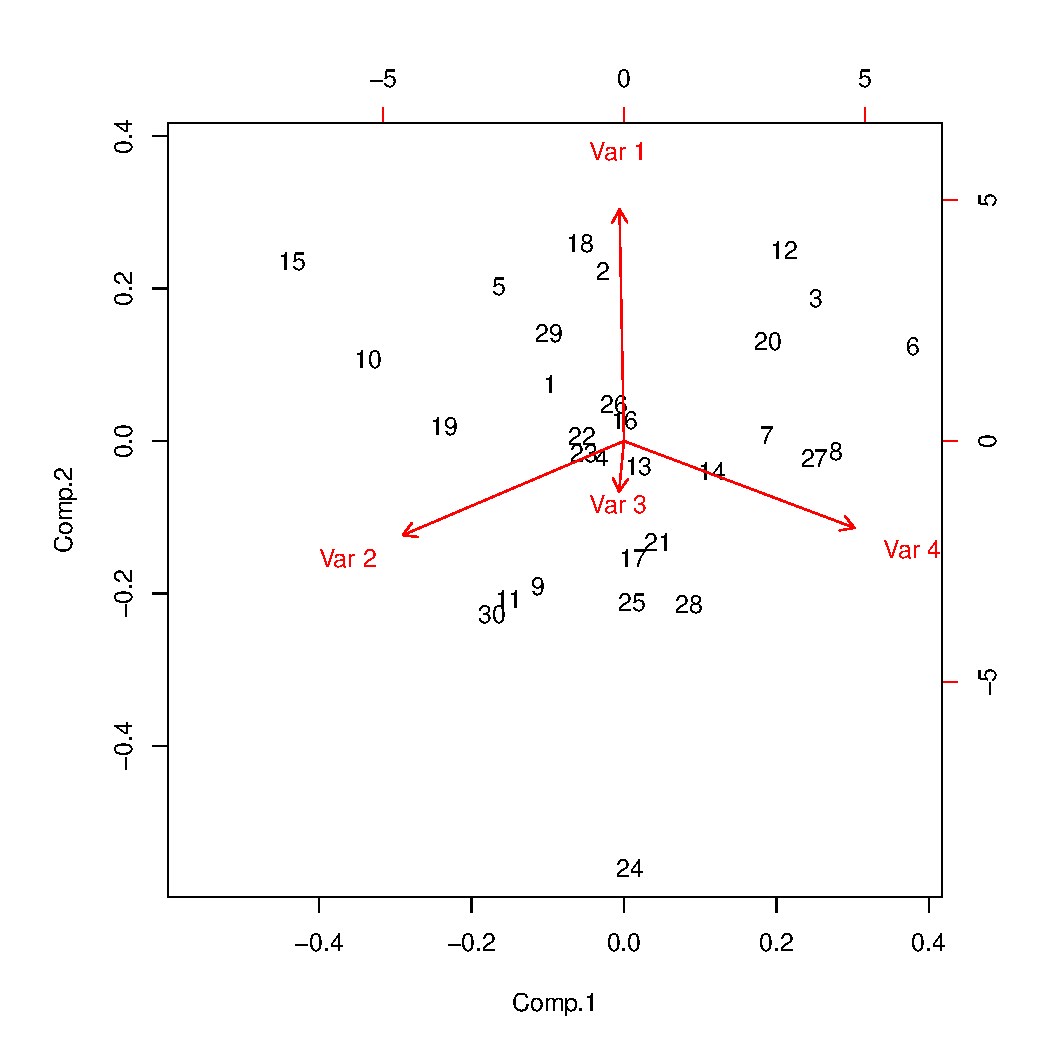
\includegraphics[width=\maxwidth]{figure/unnamed-chunk-6-1} 

\end{knitrout}

\section{Other}
\begin{enumerate}
\item Test for normality as follows:
\begin{knitrout}
\definecolor{shadecolor}{rgb}{0.969, 0.969, 0.969}\color{fgcolor}\begin{kframe}
\begin{alltt}
\hlcom{## This chunk was last ran in}
\hlkwd{timestamp}\hlstd{()}
\end{alltt}
\begin{verbatim}
## ##------ Wed Nov  7 09:53:39 2018 ------##
\end{verbatim}
\begin{alltt}
\hlkwd{data}\hlstd{(two_normal_pops)}
\end{alltt}


{\ttfamily\noindent\color{warningcolor}{\#\# Warning in data(two\_normal\_pops): data set 'two\_normal\_pops' not found}}\begin{alltt}
\hlkwd{par}\hlstd{(}\hlkwc{mfrow}\hlstd{=}\hlkwd{c}\hlstd{(}\hlnum{1}\hlstd{,}\hlnum{2}\hlstd{))}
\hlkwd{qqnorm.acomp}\hlstd{(}\hlkwd{acomp}\hlstd{(two_normal_pops}\hlopt{@}\hlkwc{count_matrix}\hlstd{),} \hlkwc{pch}\hlstd{=}\hlnum{19}\hlstd{,} \hlkwc{cex}\hlstd{=}\hlnum{0.2}\hlstd{)}
\end{alltt}


{\ttfamily\noindent\bfseries\color{errorcolor}{\#\# Error in acomp(two\_normal\_pops@count\_matrix): object 'two\_normal\_pops' not found}}\begin{alltt}
\hlkwd{qqnorm.acomp}\hlstd{(}\hlkwd{acomp}\hlstd{(two_normal_pops}\hlopt{@}\hlkwc{count_matrix}\hlstd{[}\hlnum{1}\hlopt{:}\hlnum{1000}\hlstd{,]),} \hlkwc{pch}\hlstd{=}\hlnum{19}\hlstd{,} \hlkwc{cex}\hlstd{=}\hlnum{0.2}\hlstd{,} \hlkwc{plot.it}\hlstd{=}\hlnum{FALSE}\hlstd{)}
\end{alltt}


{\ttfamily\noindent\bfseries\color{errorcolor}{\#\# Error in acomp(two\_normal\_pops@count\_matrix[1:1000, ]): object 'two\_normal\_pops' not found}}\end{kframe}
\end{knitrout}
\end{enumerate}

\section{Clustering of samples}



\clearpage

\subsection{Testing hypotheses about two populations}
We might have our samples split into two categories; e.g. sex. As in Aithison 1986\cite{}, I follow a hierarchy of alternative hypotheses, from least to most complex.

Our first question is whether two populations have the same covariance and structure and center (i.e. if there is any distributional difference)

\begin{knitrout}
\definecolor{shadecolor}{rgb}{0.969, 0.969, 0.969}\color{fgcolor}\begin{kframe}
\begin{alltt}
\hlcom{## This chunk was last ran in}
\hlkwd{timestamp}\hlstd{()}
\end{alltt}
\begin{verbatim}
## ##------ Wed Nov  7 09:53:40 2018 ------##
\end{verbatim}
\begin{alltt}
\hlcom{##TODO!!}
\end{alltt}
\end{kframe}
\end{knitrout}

The next is whether the populations have a different center:

\begin{knitrout}
\definecolor{shadecolor}{rgb}{0.969, 0.969, 0.969}\color{fgcolor}\begin{kframe}
\begin{alltt}
\hlcom{## This chunk was last ran in}
\hlkwd{timestamp}\hlstd{()}
\end{alltt}
\begin{verbatim}
## ##------ Wed Nov  7 09:53:40 2018 ------##
\end{verbatim}
\begin{alltt}
\hlcom{## This dataset includes the two components above, as well as four others}
\hlcom{## (a total of seven)}
\hlkwd{data}\hlstd{(}\hlstr{"two_normal_pops_extended"}\hlstd{)}
\end{alltt}


{\ttfamily\noindent\color{warningcolor}{\#\# Warning in data("{}two\_normal\_pops\_extended"{}): data set 'two\_normal\_pops\_extended' not found}}\begin{alltt}
\hlcom{## Data from the Landscape... paper}
\hlkwd{data}\hlstd{(}\hlstr{"Breast560"}\hlstd{)}
\end{alltt}


{\ttfamily\noindent\color{warningcolor}{\#\# Warning in data("{}Breast560"{}): data set 'Breast560' not found}}\begin{alltt}
\hlstd{wrapper_compare_populations} \hlkwb{<-} \hlkwa{function}\hlstd{(}\hlkwc{predictors}\hlstd{,} \hlkwc{response}\hlstd{,} \hlkwc{...}\hlstd{)\{}
  \hlkwa{if}\hlstd{(}\hlkwd{length}\hlstd{(}\hlkwd{unique}\hlstd{(response))} \hlopt{==} \hlnum{2}\hlstd{)\{}
    \hlstd{tmp} \hlkwb{<-} \hlkwd{compare_populations}\hlstd{(predictors, response, ...)}
    \hlstd{tmp} \hlkwb{<-} \hlstd{tmp}\hlopt{$}\hlstd{info[}\hlnum{1}\hlopt{:}\hlnum{2}\hlstd{]}
    \hlstd{tmp}
  \hlstd{\}}
\hlstd{\}}

\hlstd{x} \hlkwb{<-} \hlkwd{do.call}\hlstd{(}\hlstr{'rbind'}\hlstd{,} \hlkwd{lapply}\hlstd{(}\hlnum{1}\hlopt{:}\hlkwd{ncol}\hlstd{(}\hlkwd{metadata}\hlstd{(Breast560)),}
       \hlkwa{function}\hlstd{(}\hlkwc{k}\hlstd{)\{}
         \hlkwd{wrapper_compare_populations}\hlstd{(}\hlkwc{predictors} \hlstd{=} \hlkwd{count_matrix}\hlstd{(Breast560),}
                                     \hlkwc{response} \hlstd{=} \hlkwd{metadata}\hlstd{(Breast560)[,k])}
         \hlstd{\}}
       \hlstd{))}
\end{alltt}


{\ttfamily\noindent\bfseries\color{errorcolor}{\#\# Error in metadata(Breast560): object 'Breast560' not found}}\begin{alltt}
\hlstd{x}
\end{alltt}


{\ttfamily\noindent\bfseries\color{errorcolor}{\#\# Error in eval(expr, envir, enclos): object 'x' not found}}\end{kframe}
\end{knitrout}


\section{Data for 560 breast cancer patients}
Data from 560 breast cancer patients is available as part of the document as well:

\begin{knitrout}
\definecolor{shadecolor}{rgb}{0.969, 0.969, 0.969}\color{fgcolor}\begin{kframe}
\begin{alltt}
\hlkwd{data}\hlstd{(}\hlstr{"Breast560"}\hlstd{)}
\end{alltt}


{\ttfamily\noindent\color{warningcolor}{\#\# Warning in data("{}Breast560"{}): data set 'Breast560' not found}}\begin{alltt}
\hlkwd{metadata}\hlstd{(Breast560)[}\hlnum{1}\hlopt{:}\hlnum{4}\hlstd{,}\hlnum{1}\hlopt{:}\hlnum{5}\hlstd{]}
\end{alltt}


{\ttfamily\noindent\bfseries\color{errorcolor}{\#\# Error in metadata(Breast560): object 'Breast560' not found}}\begin{alltt}
\hlkwd{count_matrix}\hlstd{(Breast560)[}\hlnum{1}\hlopt{:}\hlnum{4}\hlstd{,}\hlnum{1}\hlopt{:}\hlnum{5}\hlstd{]}
\end{alltt}


{\ttfamily\noindent\bfseries\color{errorcolor}{\#\# Error in count\_matrix(Breast560): object 'Breast560' not found}}\end{kframe}
\end{knitrout}

Not sure if this is correct
\begin{knitrout}
\definecolor{shadecolor}{rgb}{0.969, 0.969, 0.969}\color{fgcolor}\begin{kframe}
\begin{alltt}
\hlkwd{source}\hlstd{(}\hlstr{"~/Documents/CantabPhD/CDA_in_Cancer/code/functions/various_functions.R"}\hlstd{)}
\end{alltt}


{\ttfamily\noindent\color{warningcolor}{\#\# Warning in file(filename, "{}r"{}, encoding = encoding): cannot open file '/Users/morril01/Documents/CantabPhD/CDA\_in\_Cancer/code/functions/various\_functions.R': No such file or directory}}

{\ttfamily\noindent\bfseries\color{errorcolor}{\#\# Error in file(filename, "{}r"{}, encoding = encoding): cannot open the connection}}\begin{alltt}
\hlkwd{plotPCA}\hlstd{(}\hlkwd{ilr}\hlstd{(}\hlkwd{count_matrix}\hlstd{(Breast560)),} \hlkwc{pch}\hlstd{=}\hlnum{4}\hlstd{,} \hlkwc{col}\hlstd{=}\hlstr{'blue'}\hlstd{)}
\end{alltt}


{\ttfamily\noindent\bfseries\color{errorcolor}{\#\# Error in plotPCA(ilr(count\_matrix(Breast560)), pch = 4, col = "{}blue"{}): could not find function "{}plotPCA"{}}}\end{kframe}
\end{knitrout}

\subsection{(ongoing) test for equality}

\begin{knitrout}
\definecolor{shadecolor}{rgb}{0.969, 0.969, 0.969}\color{fgcolor}\begin{kframe}
\begin{alltt}
\hlkwd{comp.test}\hlstd{(}\hlkwc{x} \hlstd{=} \hlkwd{count_matrix}\hlstd{(Breast560),}
                              \hlkwc{ina} \hlstd{=} \hlkwd{as.numeric}\hlstd{(}\hlkwd{as.factor}\hlstd{(}\hlkwd{metadata}\hlstd{(Breast560)}\hlopt{$}\hlstd{final.ER)),}
                              \hlkwc{test} \hlstd{=} \hlstr{"james"}\hlstd{,} \hlkwc{R} \hlstd{=} \hlnum{0}\hlstd{)}
\end{alltt}


{\ttfamily\noindent\bfseries\color{errorcolor}{\#\# Error in comp.test(x = count\_matrix(Breast560), ina = as.numeric(as.factor(metadata(Breast560)\$final.ER)), : could not find function "{}comp.test"{}}}\end{kframe}
\end{knitrout}

\section{Data for 12k TCGA samples, with ovarian cancer-derived CNA signatures}

\begin{knitrout}
\definecolor{shadecolor}{rgb}{0.969, 0.969, 0.969}\color{fgcolor}\begin{kframe}
\begin{alltt}
\hlkwd{timestamp}\hlstd{()}
\end{alltt}
\begin{verbatim}
## ##------ Wed Nov  7 09:53:40 2018 ------##
\end{verbatim}
\begin{alltt}
\hlkwd{data}\hlstd{(}\hlstr{"CNA_12K_TCGA"}\hlstd{)}
\end{alltt}


{\ttfamily\noindent\color{warningcolor}{\#\# Warning in data("{}CNA\_12K\_TCGA"{}): data set 'CNA\_12K\_TCGA' not found}}\begin{alltt}
\hlkwd{dim}\hlstd{(}\hlkwd{metadata}\hlstd{(CNA_12K_TCGA))}
\end{alltt}


{\ttfamily\noindent\bfseries\color{errorcolor}{\#\# Error in metadata(CNA\_12K\_TCGA): object 'CNA\_12K\_TCGA' not found}}\begin{alltt}
\hlkwd{dim}\hlstd{(}\hlkwd{count_matrix}\hlstd{(CNA_12K_TCGA))}
\end{alltt}


{\ttfamily\noindent\bfseries\color{errorcolor}{\#\# Error in count\_matrix(CNA\_12K\_TCGA): object 'CNA\_12K\_TCGA' not found}}\end{kframe}
\end{knitrout}


\end{document}
